\chapter{Analysis} \label{Chapter:Analysis}

\section{Camera frame rate calculation}

\todo{BOOM}

\section{Power consumption modelling}

Power consumption modelling was done by measuring the average power consumption of the algorithm running under different frame rates, with frames captured from the camera module.

\todo{BOOM}

\section{Power consumption reduction analysis}

Power consumption reduction was analysed using the video datasets from CDNET, to keep input video stream consistent. However, because the frame images inside the datasets are discrete in time, the frame rate cannot be changed in great precision, results in a rough estimation of the actual performance.

Firstly, some properties of the dataset under test need to be determined, such as maximum object moving speed and minimum FPS required. This is done by evaluate the dataset without adaptive operation. During the process, the maximum distances objects moved between each frame intervals were recorded. The top $5 \%$ of the distances that are most likely due to errors were removed. \fref{ana:ada} shows the distribution of maximum moving distances after filtering in a dataset. The maximum of those value was considered as the maximum speed an object may travel in the dataset. According to the formulae described in section \ref{imp:ada:metric}, the minimum FPS requirement was then calculated. The optical flow tracking window was set to 32 pixels, as a result most minimum FPS requirements calculated were under 1 FPS. For a faster response time, the minimum FPS was set to 2 FPS.

\begin{figure}[htb]
  \centering
  \subfigure [Absolute maximum distances objects travelled between frames] {
    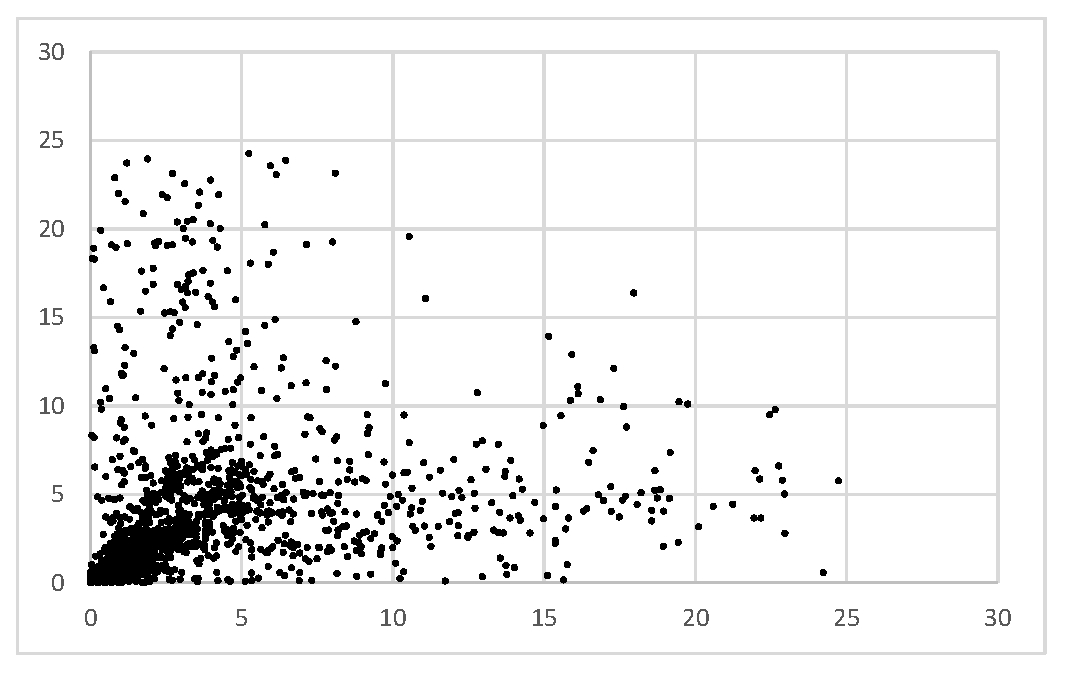
\includegraphics[width=0.45\columnwidth]{ana_ada_xy}
    \label{ana:ada:xy}
  }
  \subfigure [Histogram distribution of maximum distances] {
    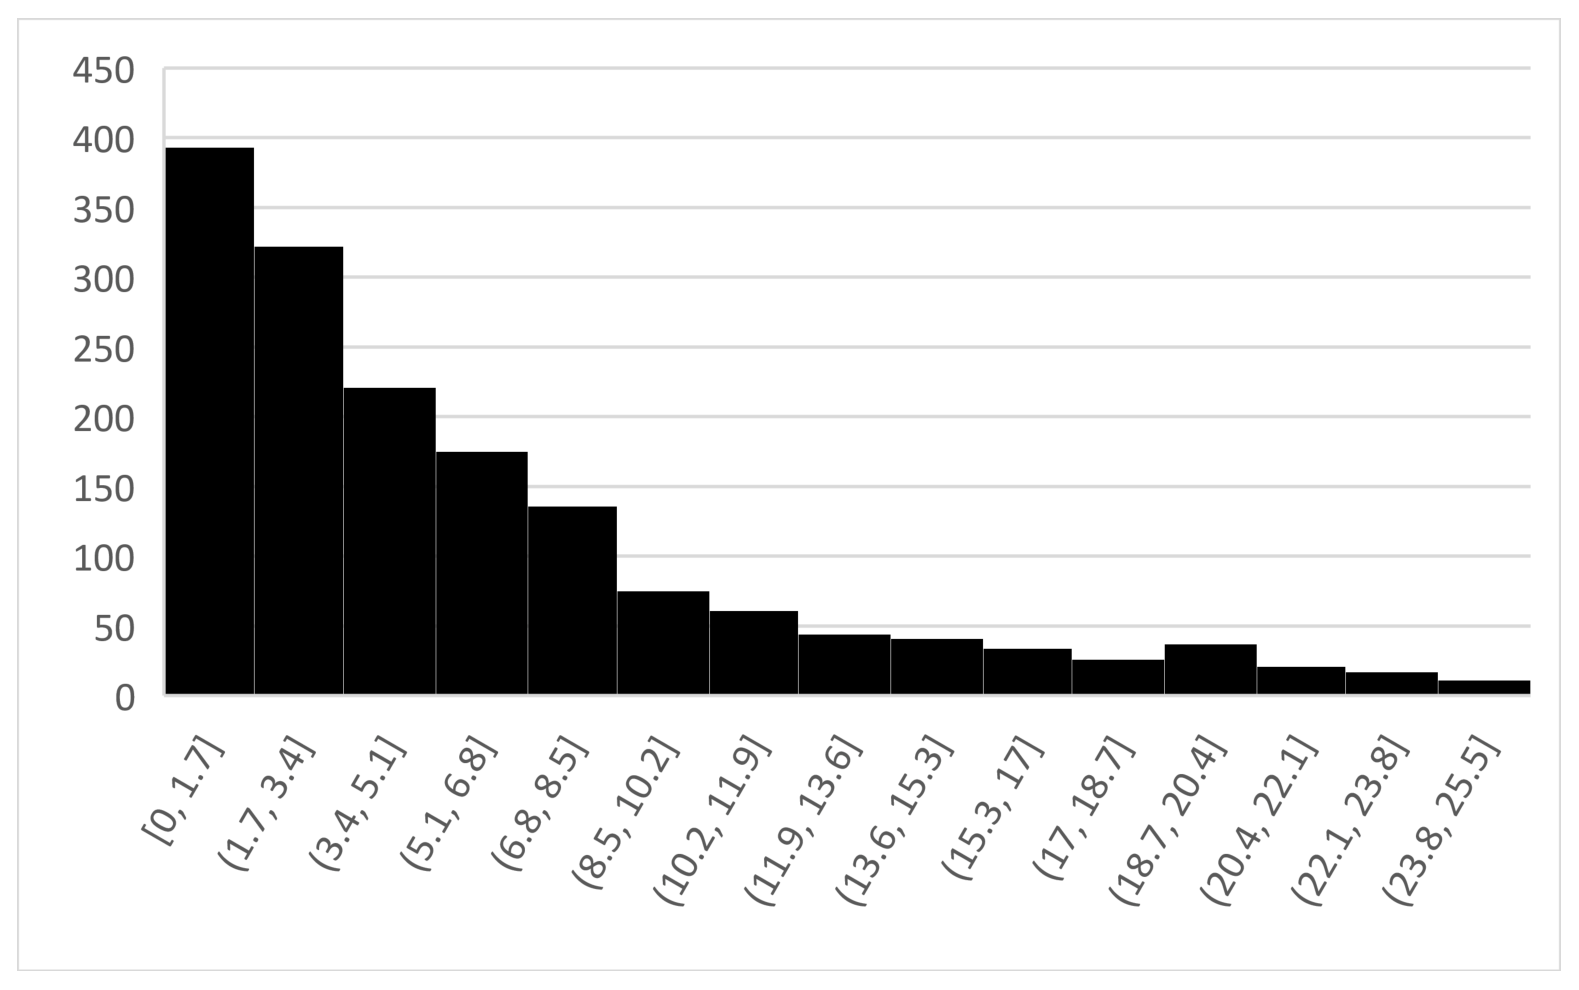
\includegraphics[width=0.45\columnwidth]{ana_ada_histo}
    \label{ana:ada:histo}
  }
  \caption{Filtered distributions from CDNET highway dataset.}
  \label{ana:ada}
\end{figure}

By applying the power consumption model, the actual power consumption can be estimated.

\begin{figure}[htb]
  \centering
  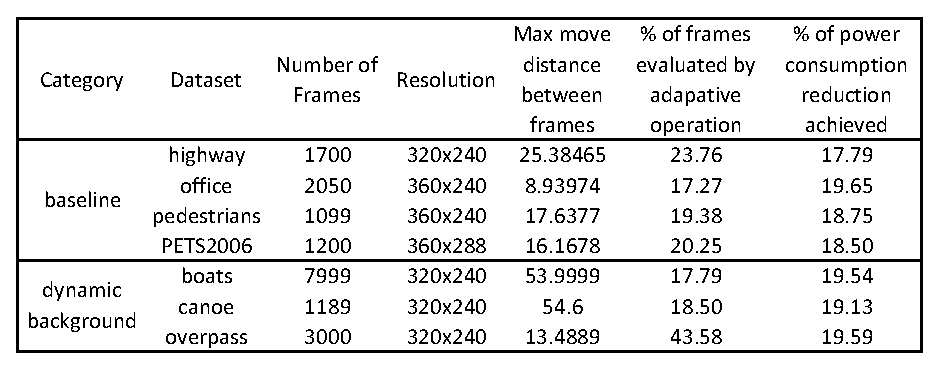
\includegraphics[width=\columnwidth]{ana_summary}
  \caption{Summary of evaluated CDNET datasets.}
  \label{ana:summary}
\end{figure}

\todo{BOOM}
